\documentclass[ 12pt,a4paper,twocolumn,fleqn]{article}
\usepackage{graphicx}
\usepackage[a4paper,top=20mm, bottom=30mm, left=10mm, right=25mm]{geometry}
\usepackage{fancyhdr}
\usepackage{hyperref}
\usepackage{listings}
\usepackage[]{algorithm2e}
\usepackage{color}
\usepackage{fancybox}
\thisfancypage{%
  \setlength{\fboxsep}{20pt}\doublebox}{}
\pagestyle{fancy}
\usepackage{lineno}
\usepackage{xtab,booktabs}
\usepackage{setspace}
\usepackage{amsmath}
\usepackage{xcolor}
\usepackage{graphicx}
\usepackage{subcaption}
\usepackage{graphicx}
\usepackage{tikz}
\usepackage[compact]{titlesec}
\titlespacing{\section}{0pt}{*0}{*0}
\titlespacing{\subsection}{0pt}{*0}{*0}
\titlespacing{\subsubsection}{0pt}{*0}{*0}
\setlength\columnsep{25pt}
\makeatletter
\g@addto@macro{\normalsize}{%
\setlength{\abovedisplayskip}{0pt}
\setlength{\abovedisplayshortskip}{0pt}
\setlength{\belowdisplayskip}{0pt}
\setlength{\belowdisplayshortskip}{0pt}}
\makeatother
\mathindent=0.0pt
\usepackage{float}
\renewcommand{\baselinestretch}{1.5}
\begin{document}
\lhead{Header Title is here...}
\chead{}

\onecolumn
\begin{center}
\textcolor{brown}{\LARGE{INDEPENDENT UNIVERSITY, BANGLADESH}} \\

\includegraphics[scale=0.5]{media/IUB.png} \\

%\large{\textbf{Bachelor of Technology}} \\
%\large{in} \\
\large{Computer Science and Engineering} \\
\large{School of Engineering, Technology and Sciences} \\

%\includegraphics[width=0.18\textwidth]{media/Logo of AIML.jpeg.jpg}

\text{A Project Report On} \\
\smallskip
\textcolor{cyan}{\LARGE{TITLE}} \\



\textit{Submitted By} \\
\textbf{Name1, \space ID} \\
\textbf{Name2, \space ID} \\

\textit{Under the guidance of} \\
\textbf{Md Masum Billah} \\
\text{Assistant Professor, CSE, IUB}\\
\large{\textbf{Summer: 2026}} \\
\textcolor{blue}{\large{Department of Computer Science and Engineering }} \\
\textcolor{blue}{\large{INDEPENDENT UNIVERSITY, BANGLADESH}} \\
\textcolor{blue}{\large{DHAKA}} \\
\end{center}

\newpage
  \pagestyle{fancy}
\thisfancypage{%
  \setlength{\fboxsep}{20pt}\doublebox}{}



% Latex code for adding double lined box for pages
% Should add this code for every page
\newpage
  \pagestyle{fancy}
\thisfancypage{%
  \setlength{\fboxsep}{20pt}\doublebox}{}
  
\begin{center}
\LARGE{{\underline{Acknowledgement}}} \\
\end{center}
\normalsize

Here writing your acknowledgement.......
\begin{flushright}
\begin{centering}
    \textbf{Student 1 \space ID} \\
\textbf{Student 2 \space ID} \\

\end{centering}

\end{flushright}


\newpage
  \pagestyle{fancy}
\thisfancypage{%
  \setlength{\fboxsep}{20pt}\doublebox}{}
  
\setstretch{1.5}
\twocolumn[
\begin{@twocolumnfalse}
\title {Our Project title }
\date{}
\author{Student 1, Student 2,}
\maketitle



{\bfseries\LARGE Abstract} \\
    
Project abstract is here......


\end{@twocolumnfalse}]
\modulolinenumbers[5]
\onecolumn
\newpage
  \pagestyle{fancy}
\thisfancypage{%
  \setlength{\fboxsep}{20pt}\doublebox}{}
\tableofcontents
\newpage
  \pagestyle{fancy}
\thisfancypage{%
  \setlength{\fboxsep}{20pt}\doublebox}{}
\newpage
  \pagestyle{fancy}
\thisfancypage{%
  \setlength{\fboxsep}{20pt}\doublebox}{}
  
\section{Introduction}
Reinforcement Learning (RL) \cite{b1} stands as a pivotal methodology in the Artificial........

\subsection{Scope}
Write the scope of your project

\section{Problem Definition}


\section{Literature Review}

\section{Methodology}

\subsection{Data Collection}

\subsection{Data Pre-processing}

\subsection{Model Implementation}

\subsubsection{Logistic Regression}

\section{Requirements}

\subsection{Functional Requirements}
\begin{itemize}
\item Requirement 1
\item Requirement 2
\item Requirement 3
\end{itemize}


\subsection{Non- Functional Requirements}
\begin{itemize}
\item Requirement 1
\item Requirement 2
\item Requirement 3
\end{itemize}

\clearpage

\newpage
 \pagestyle{fancy}
\thisfancypage{%
  \setlength{\fboxsep}{20pt}\doublebox}{}

\section{Results \& Analysis}

\begin{figure}[h]
    \centering
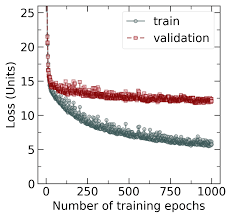
\includegraphics[width=0.5\textwidth]{media/sample.png}
    \caption{Your Image Caption}
    \label{fig:your_image}
\end{figure}

\clearpage

\newpage
 \pagestyle{fancy}
\thisfancypage{%
  \setlength{\fboxsep}{20pt}\doublebox}{}
  
\section{Conclusion \& Future work}

\clearpage

\newpage
 \pagestyle{fancy}
\thisfancypage{%
  \setlength{\fboxsep}{20pt}\doublebox}{}

\section{References}
% Include your references here
\begin{thebibliography}{9}

\bibitem{b1}
Chan, Stephanie CY, et al. "Measuring the reliability of reinforcement learning algorithms." arXiv preprint arXiv:1912.05663 (2019).

\bibitem{b2}
Louis, Ruwaid, and David Yu. "A study of the exploration/exploitation trade-off in reinforcement learning: Applied to autonomous driving." (2019). \\
\url{https://www.diva-portal.org/smash/get/diva2:1336430/FULLTEXT01.pdf}

\end{thebibliography}

\end{document}
